\section{Introduction}

\begin{frame}
    \frametitle{Why Distribution?}
    \begin{itemize}
        \item Economics \\
            - Much better price/performance ratio
        \item Reliablity \\
            - One node fails, but the service goes on
        \item Enhanced performance \\
            - Tasks can be executed concurrently
        \item Easier modular expansion \\
            - Hardware and software resources can be easily added without replacing existing resources.
        \item Resource Sharing \\
            - Only one printer, share it over the network
    \end{itemize}
\end{frame}

\begin{frame}
    \frametitle{What is a Distributed system?}
    \begin{block}{Definition}
    A distributed system consists of a \alert{collection of autonomous computers}, connected through a \alert{network} and distribution \alert{middleware}, which enables computers to coordinate their activities and to share the resources of the system, so that users perceive the system as single, integrated computing facility.
    \end{block}
    \begin{columns}
        \column{.6\textwidth}
            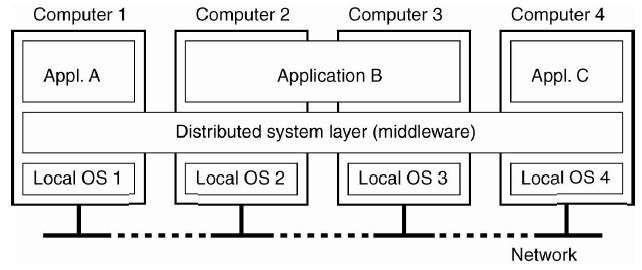
\includegraphics[scale=0.4]{dist-arch.png}
        \column{.4\textwidth}
            \begin{itemize}
                \item Resource Sharing
                \item Transparency
                \item Scalability
                \item Concurrency
                \item Fault Tolerance
            \end{itemize}
        \end{columns}
\end{frame}

\begin{frame}[allowframebreaks]
    \frametitle{Typical Distributed Systems}
    \begin{itemize}
        \item Distributed Storage System
        \begin{itemize}
            \item Structured Storage Systems
            \begin{itemize}
                \item MySQL, PostgreSQL
                \item Structured data
                \item Strong consistency
                \item Random access
                \item Expansion not good
            \end{itemize}
            \item No-Structed Storage Systems
            \begin{itemize}
                \item GFS, HDFS
                \item Manage data using metadata by master
                \item Big chunks(like 64MB), replicated copy
                \item Fault tolerant automatically.
                \item No random access, typically append
                \item Not good for real-time system
            \end{itemize}
            \item Semi-Structure Storage Systems
            \begin{itemize}
                \item NoSQL(Bigtable, Dynamo, Habse)
                \item Good Expansion
                \item Random access(update, read)
                \item Key-Value Store, No SQL, No ACID
            \end{itemize}
            \item In-memory Storage Systems
            \begin{itemize}
                \item memcached, redis
                \item based on memory, not disk.
            \end{itemize}
            \item NewSQL
            \begin{itemize}
                \item Spanner
                \item Use atomic clock to realize syncronization
                \item both expansion and SQL
            \end{itemize}
        \end{itemize}
        \item Distributed Computing System
        \begin{itemize}
            \item MapReduce like: MapReduce(Hadoop), Spark
            \item Graph: GraphLab, Pregel
            \item Streaming: Storm
        \end{itemize}
        \item \ldots
    \end{itemize}
\end{frame}

\begin{frame}
    \frametitle{Topic: Performance}
    \begin{block}{The dream: scalable throughput}
        Nx servers -> Nx total throughput via parallel CPU/disk/net. \\
        So handling more load only requires buying more computers.
    \end{block}
    Scaling gets harder as N grows:
    \begin{itemize}
        \item Load im-balance, stragglers.
        \item Non-parallelizable code: initialization, interaction.
        \item Bottlenecks from shared resources, e.g. network.
    \end{itemize}
\end{frame}

\begin{frame}
    \frametitle{Topic: Fault Tolerance}
    \begin{itemize}
        \item 1000s of servers, complex net -> always something broken.
        \item We'd like to hide these failures from the application.
        \item We ofen want:
        \begin{itemize}
            \item Availability  -- app can keep using its data despite failures. \\
            \item Durability -- app's data will come back to life when failures are repaired. \\
        \end{itemize}
        \item Big idea: replicated servers. \\
        If one server crashes, client can proceed using the other(s).
    \end{itemize}
\end{frame}

\begin{frame}
    \frametitle{Topic: Consistency}
    \begin{itemize}
        \item General-purpose infrastructure needs well-defined behavior. \\
            E.g. 'Get(k) yields the value from the most recent Put(k,v)'
        \item Achieving good behavior is hard!
        \begin{itemize}
            \item 'Replica' servers are hard to keep identical.
            \item Clients may crash midway through multi-step update.
            \item Servers crash at awkward moments. e.g. after executing but before replying.
            \item Network may make live servers look dead.
        \end{itemize}
        \item Consistency and performance are enemies.
        \begin{itemize}
            \item Consistency requires communication, e.g. to get latest Put().
            \item \alert{Strong Consistency} often leads to slow systems.
            \item High performance often imposes \alert{weak consistency} on applications.
        \end{itemize}
    \end{itemize}
\end{frame}

\begin{frame}
    \frametitle{Later\ldots}
    \begin{itemize}
        \item Lamport's Logic Clock
        \item P2P Systems
        \item Leader Election
        \item Concensus Algorithm
        \item \ldots
    \end{itemize}
\end{frame}
